% Angström Ang
\newcommand{\Ang}{{\hspace{.2em}}\text{\AA}}

%-----------------------------------------------------------

\section[k-point sampling in the Brillouin zone for semiconductors]{$k$-point sampling in the Brillouin zone for semiconductors}
\label{sec:k-point-sampling}

In a semiconductor, the choice of the $k$-grid is crucial for accurately sampling the Brillouin zone, because the valence band maxima (VBM) and conduction band minima (CBM) are usually located at high symmetry points. Here, we describe three different choices for a $k$-grid offset:
\begin{itemize}
 \item a $\Gamma$-centered grid,
 \item the grid suggested by Monkhorst and Pack \cite{Monkhorst76} and
 \item an off-$\Gamma$ grid.
\end{itemize}

They are defined as
\begin{equation}
  \label{eqn_K-shift}
  u_{r}=\begin{cases}
\frac{r-q}{q}& \text{$\Gamma$-centered},\\
\frac{2r-q-1}{2q}& \text{Monkhorst-Pack},\\
\frac{r-1}{q}+\frac{1}{2q}& \text{off-$\Gamma$}
\end{cases}
\end{equation}
where $r=1 \dotsc q$ and $q$ is the total number of points. In
Fig.~(\ref{fig:G-centered}, \ref{fig:MP_grid} and \ref{fig:off-gamma_grid})
the three different shifts are illustrated. The Monkhorst-Pack grid\footnote{%
  One could argue that Monkhorst and Pack never intended their formula to be
  used for for odd $q$.  Still, for the sake of this section,
  ``Monkhorst-Pack'' refers to this definition.} %
agrees with the $\Gamma$-centered grid for an uneven number of grid points and
with the off$-\Gamma$ grid for an even number of points. The $\Gamma$-centered
grid and sequentially the Monkhorst-Pack grid with an uneven number of grid
points include the $\Gamma$-point.\\
%
To achieve the relevant settings in the \texttt{control.in} file, two keywords have to be changed. For the number of grid points the keyword \keyword{k\_grid} needs to be specified:\\
\keyword{k\_grid} \option{n1} \option{n2} \option{n3},\\
where the numbers $n_1,~n_2,~n_3$ are integers defining the number of splits along the reciprocal vectors.\\
For the off-$\Gamma$ and Monkhorst-Pack shift, a second keyword has to be given in the \texttt{control.in} file:\\
\keyword{k\_offset} \option{f1} \option{f2} \option{f3},\\
where \option{fi} are fractional coordinates between zero and one. The offset can be defined according to Eqn.~(\ref{case_koffset}).
%
\begin{equation}
 \text{k\_offset}~ \begin{cases}
0.0 ~~ 0.0 ~~ 0.0 & \text{$\Gamma$-centered},\\
\frac{1}{2}-\frac{1}{2n_1} ~~ \frac{1}{2}-\frac{1}{2n_2} ~~ \frac{1}{2}-\frac{1}{2n_3} & \text{Monkhorst-Pack},\\
\frac{1}{2n_1} ~~ \frac{1}{2n_2} ~~ \frac{1}{2n_3} & \text{off-$\Gamma$}
\end{cases}
\end{equation}\label{case_koffset}
%
\begin{figure}
\centering
  \begin{minipage}{0.95\linewidth}
    \centering
    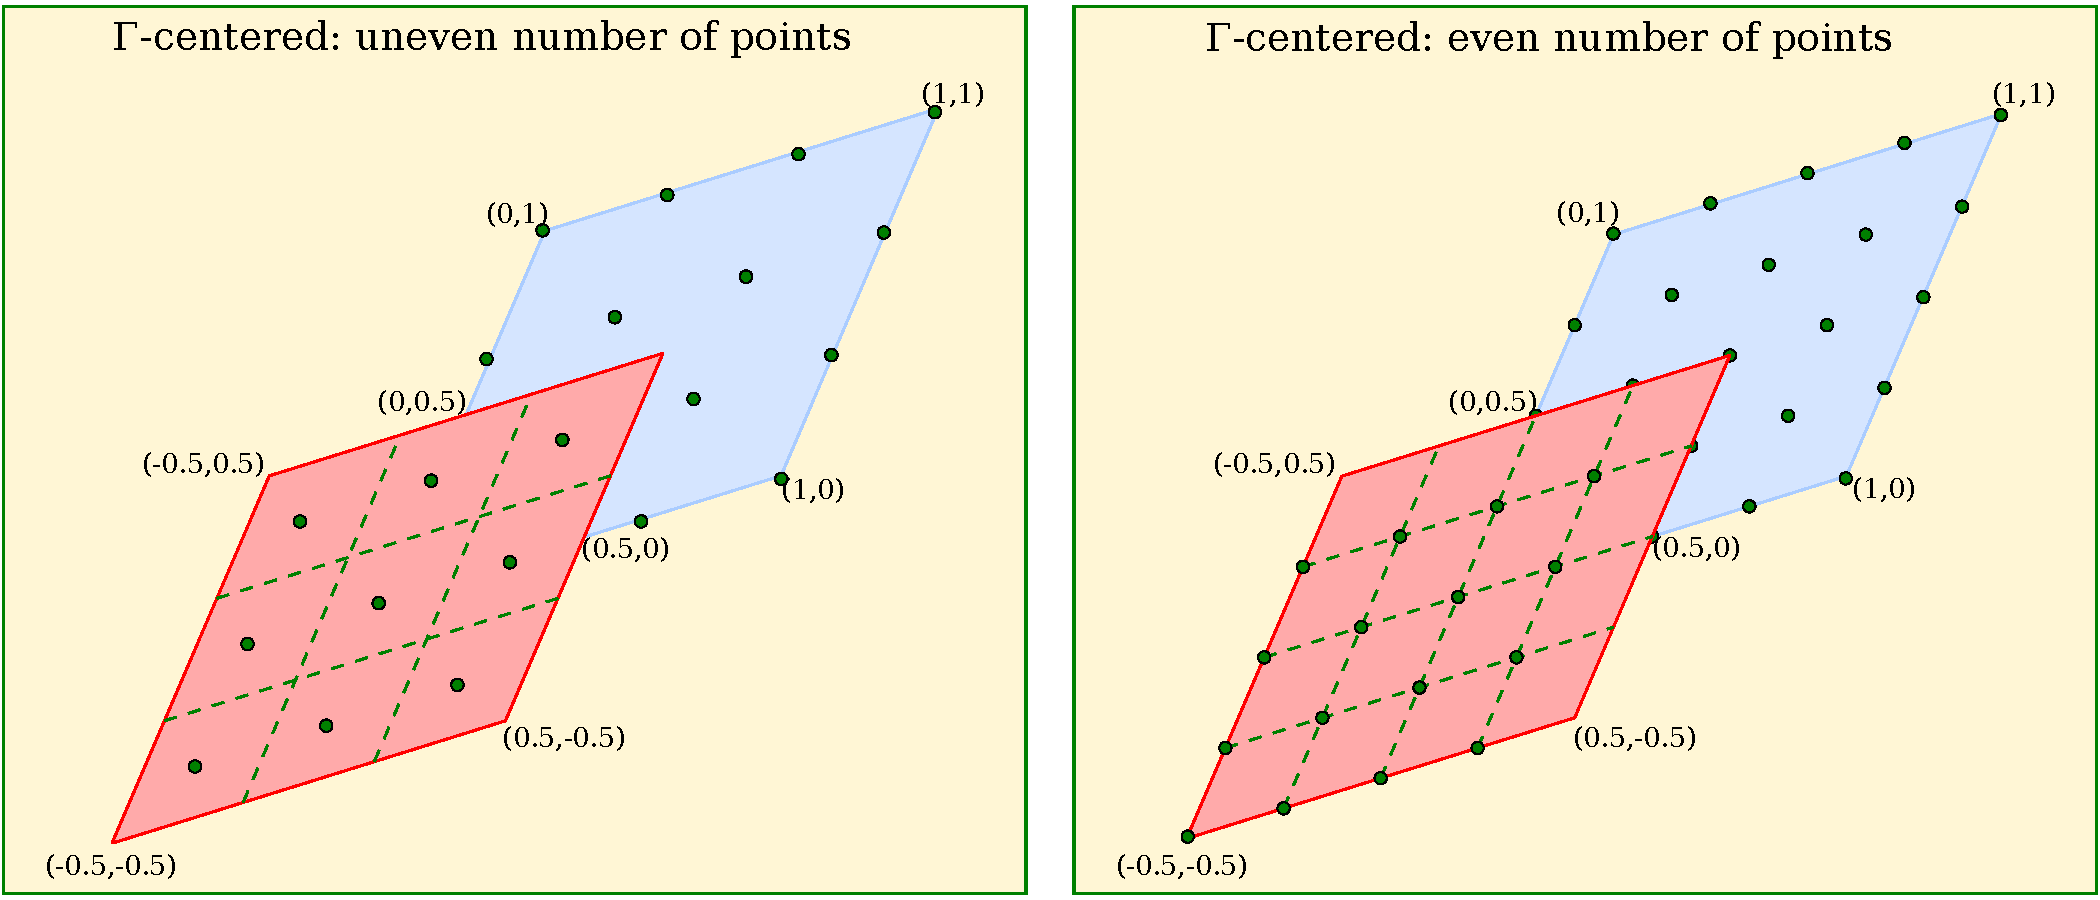
\includegraphics[width=0.90\textwidth]{./G-centered.pdf}
    % G-centered.pdf: 1008x432 pixel, 72dpi, 35.56x15.24 cm, bb=0 0 1008 432
    \caption{The $\Gamma$-centered grid in two dimensions for even and uneven numbers of grid points. In both cases the $\Gamma$-point is included in the grid.}
    \label{fig:G-centered}
  \end{minipage}
\hspace{0.0cm}
  \begin{minipage}{0.95\linewidth}
    \centering
    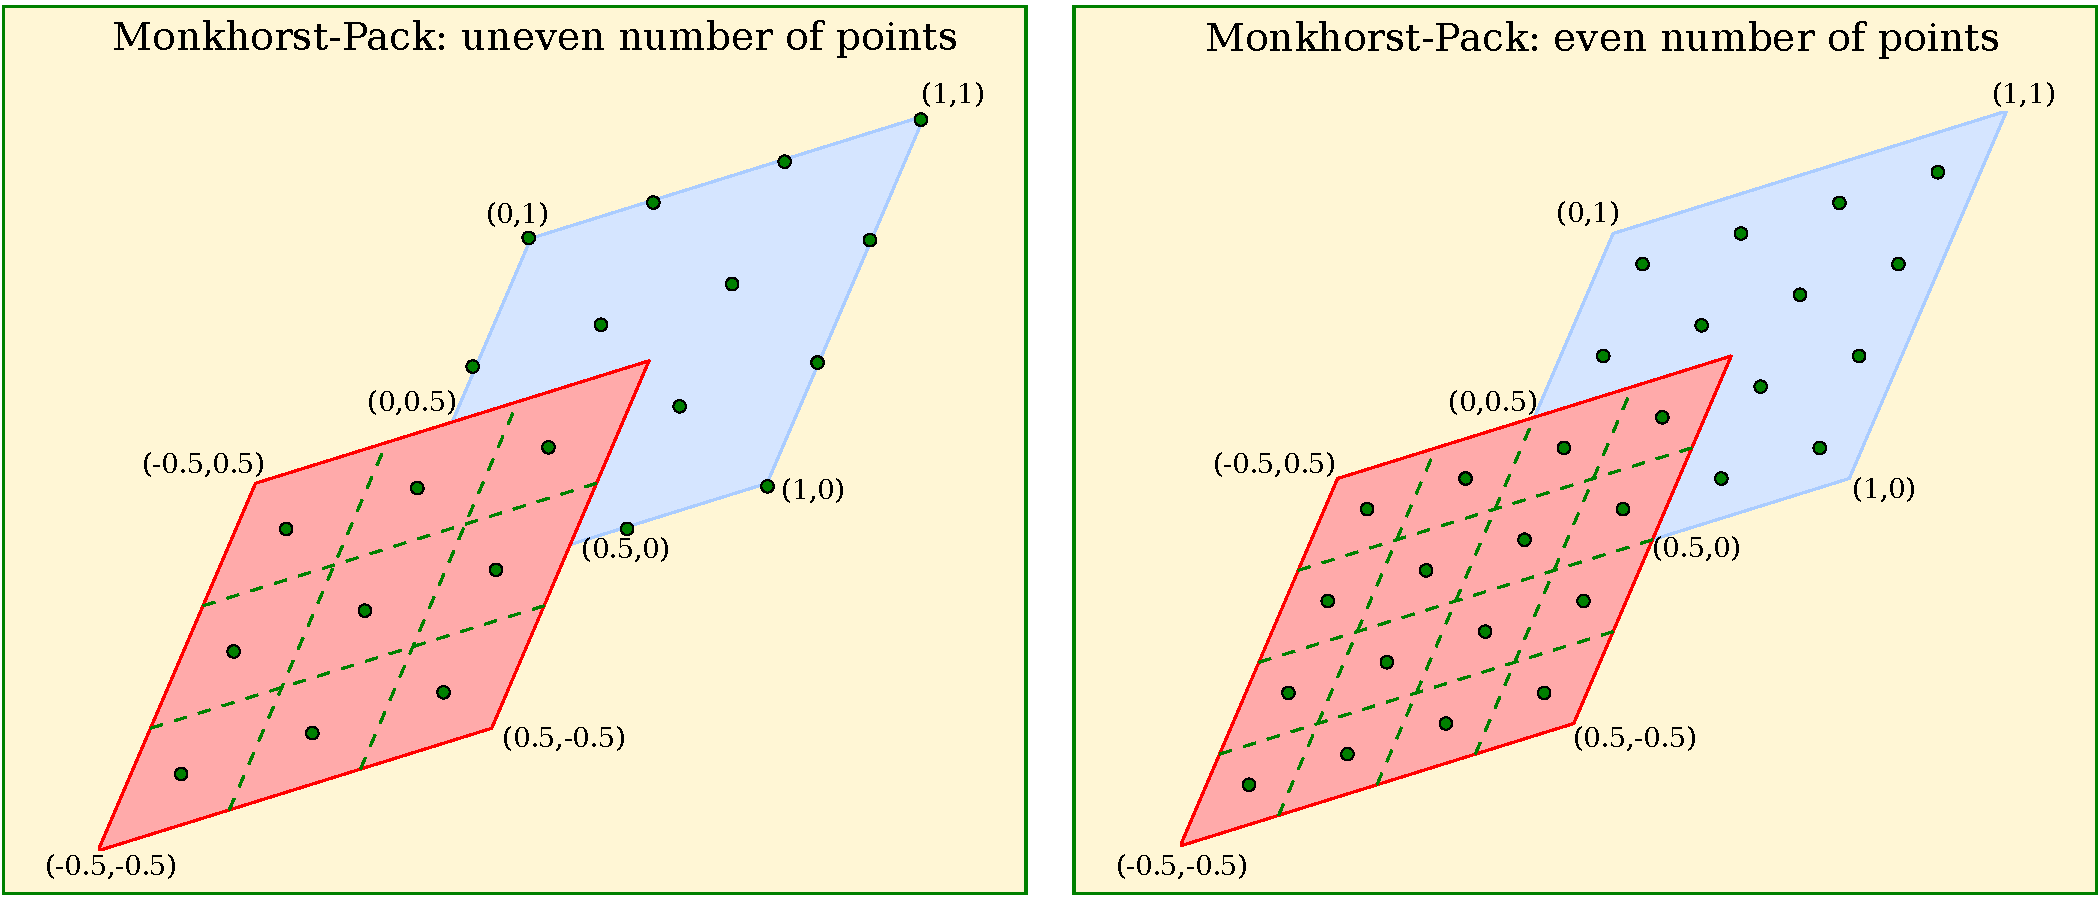
\includegraphics[width=0.90\textwidth]{./MP_grid.pdf}
    % MP_grid.pdf: 1008x432 pixel, 72dpi, 35.56x15.24 cm, bb=0 0 1008 432
    \caption{The Monkhorst Pack grid \cite{Monkhorst76} in two dimensions for even and uneven numbers of grid points. In the left picture (uneven number of grid points) the $\Gamma$ point is included in the grid.}
    \label{fig:MP_grid}
  \end{minipage}
\hspace{0.0cm}
  \begin{minipage}{0.95\linewidth}
    \centering
    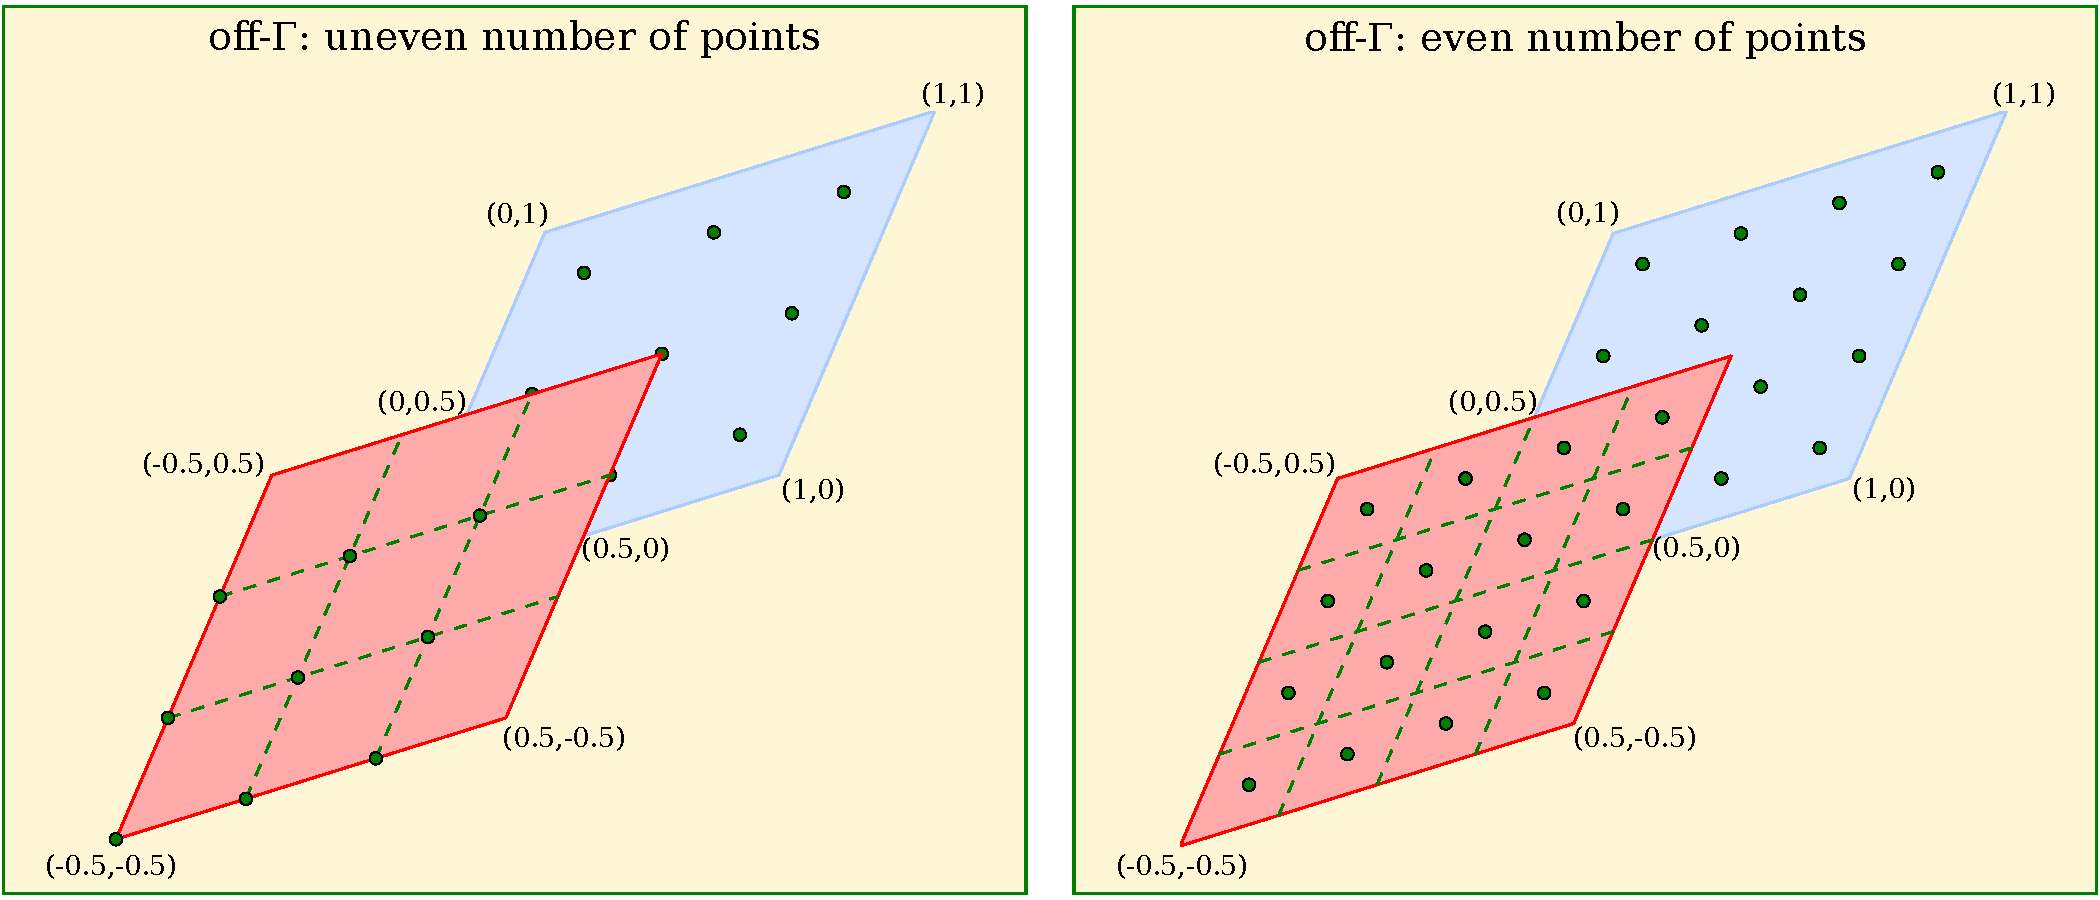
\includegraphics[width=0.90\textwidth]{./off-gamma_grid.pdf}
    % off-gamma_grid.pdf: 1008x432 pixel, 72dpi, 35.56x15.24 cm, bb=0 0 1008 432
    \caption{The off-$\Gamma$ grid in two dimensions for even and uneven numbers of grid points.}
    \label{fig:off-gamma_grid}
  \end{minipage}
\end{figure}
\clearpage
\newpage
%
\begin{wrapfigure}[12]{l}{0.33\textwidth}
\centering
 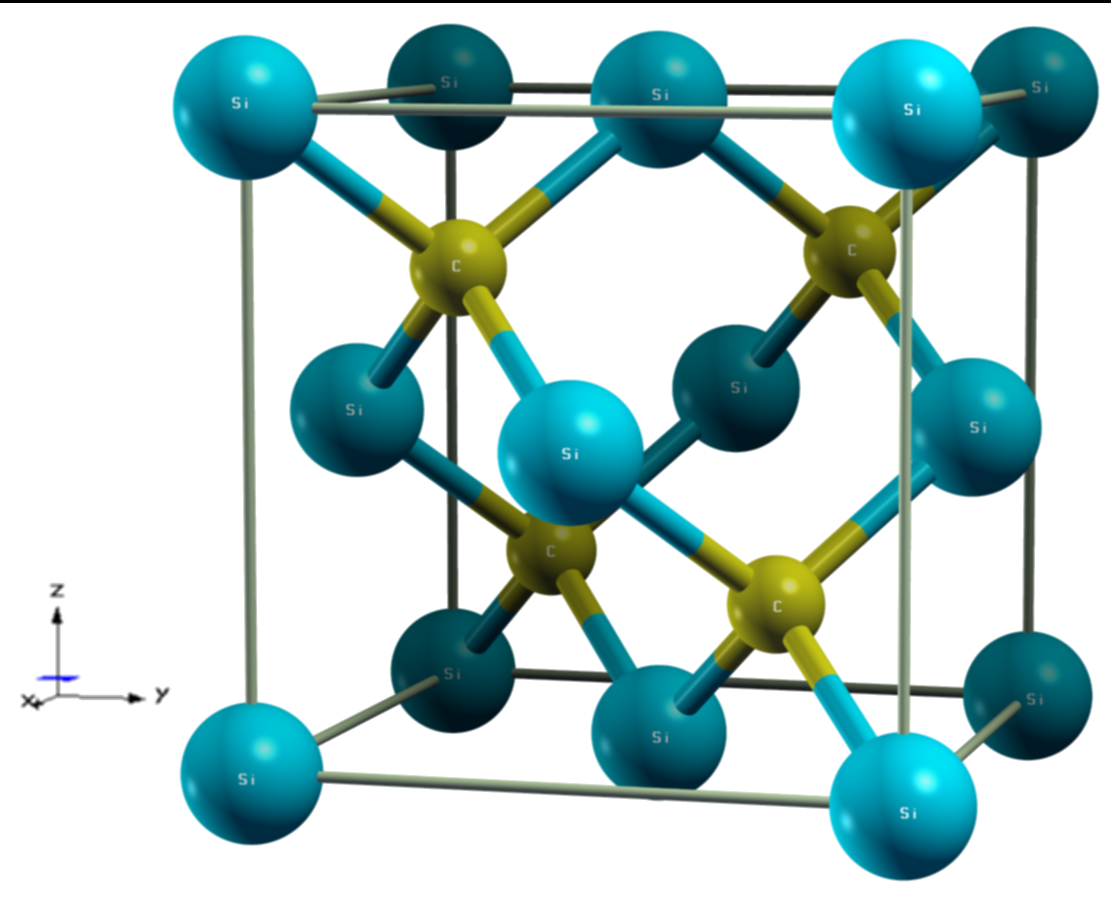
\includegraphics[width=0.30\textwidth]{./3C_SiC.png}
 % 3C_SiC.png: 1111x898 pixel, 72dpi, 39.19x31.68 cm, bb=0 0 1111 898
 \caption{The crystal structure of silicon carbide in its cubic zinc blende structure (3C-SiC)}
 \label{fig:crystal}
\end{wrapfigure}
Here,we present a concrete example. Cubic silicium carbide (3C-SiC) is a semicoductor featuring an indirect band gap between the $\Gamma$-point and the $X$-point [see Fig.~(\ref{fig:3C-SiC_bands})]. In Fig.~(\ref{fig:crystal}) the crystal structure of 3C-SiC is shown. The crystal is similar to the zinc-blende structure. The lattice constant was found to be $4.36\Ang$ \cite{itoh1997scg}.%
The $k$-grid was tested in terms of grid density in the Brillouin zone and the three different shifts discussed above.\\
As a reference energy the total energy was taken with a $k$-grid of $25 \times 25 \times 25$ $k$-points. In Fig.~(\ref{fig:aims_kgrid}) the energy differences $\left|E(k=25)-E(k) \right|$ are plotted on a logarithmic scale versus the number of $k$-points.\\%
The oscillatory behaviour in Fig.~(\ref{fig:aims_kgrid}) of the Monkhorst-Pack grid reflects the agreement with the off-$\Gamma$ grid in the case of an even number of grid points and the $\Gamma$-centered for uneven number of grid points respectively.\\
%
%
\begin{figure}[h]
\centering
 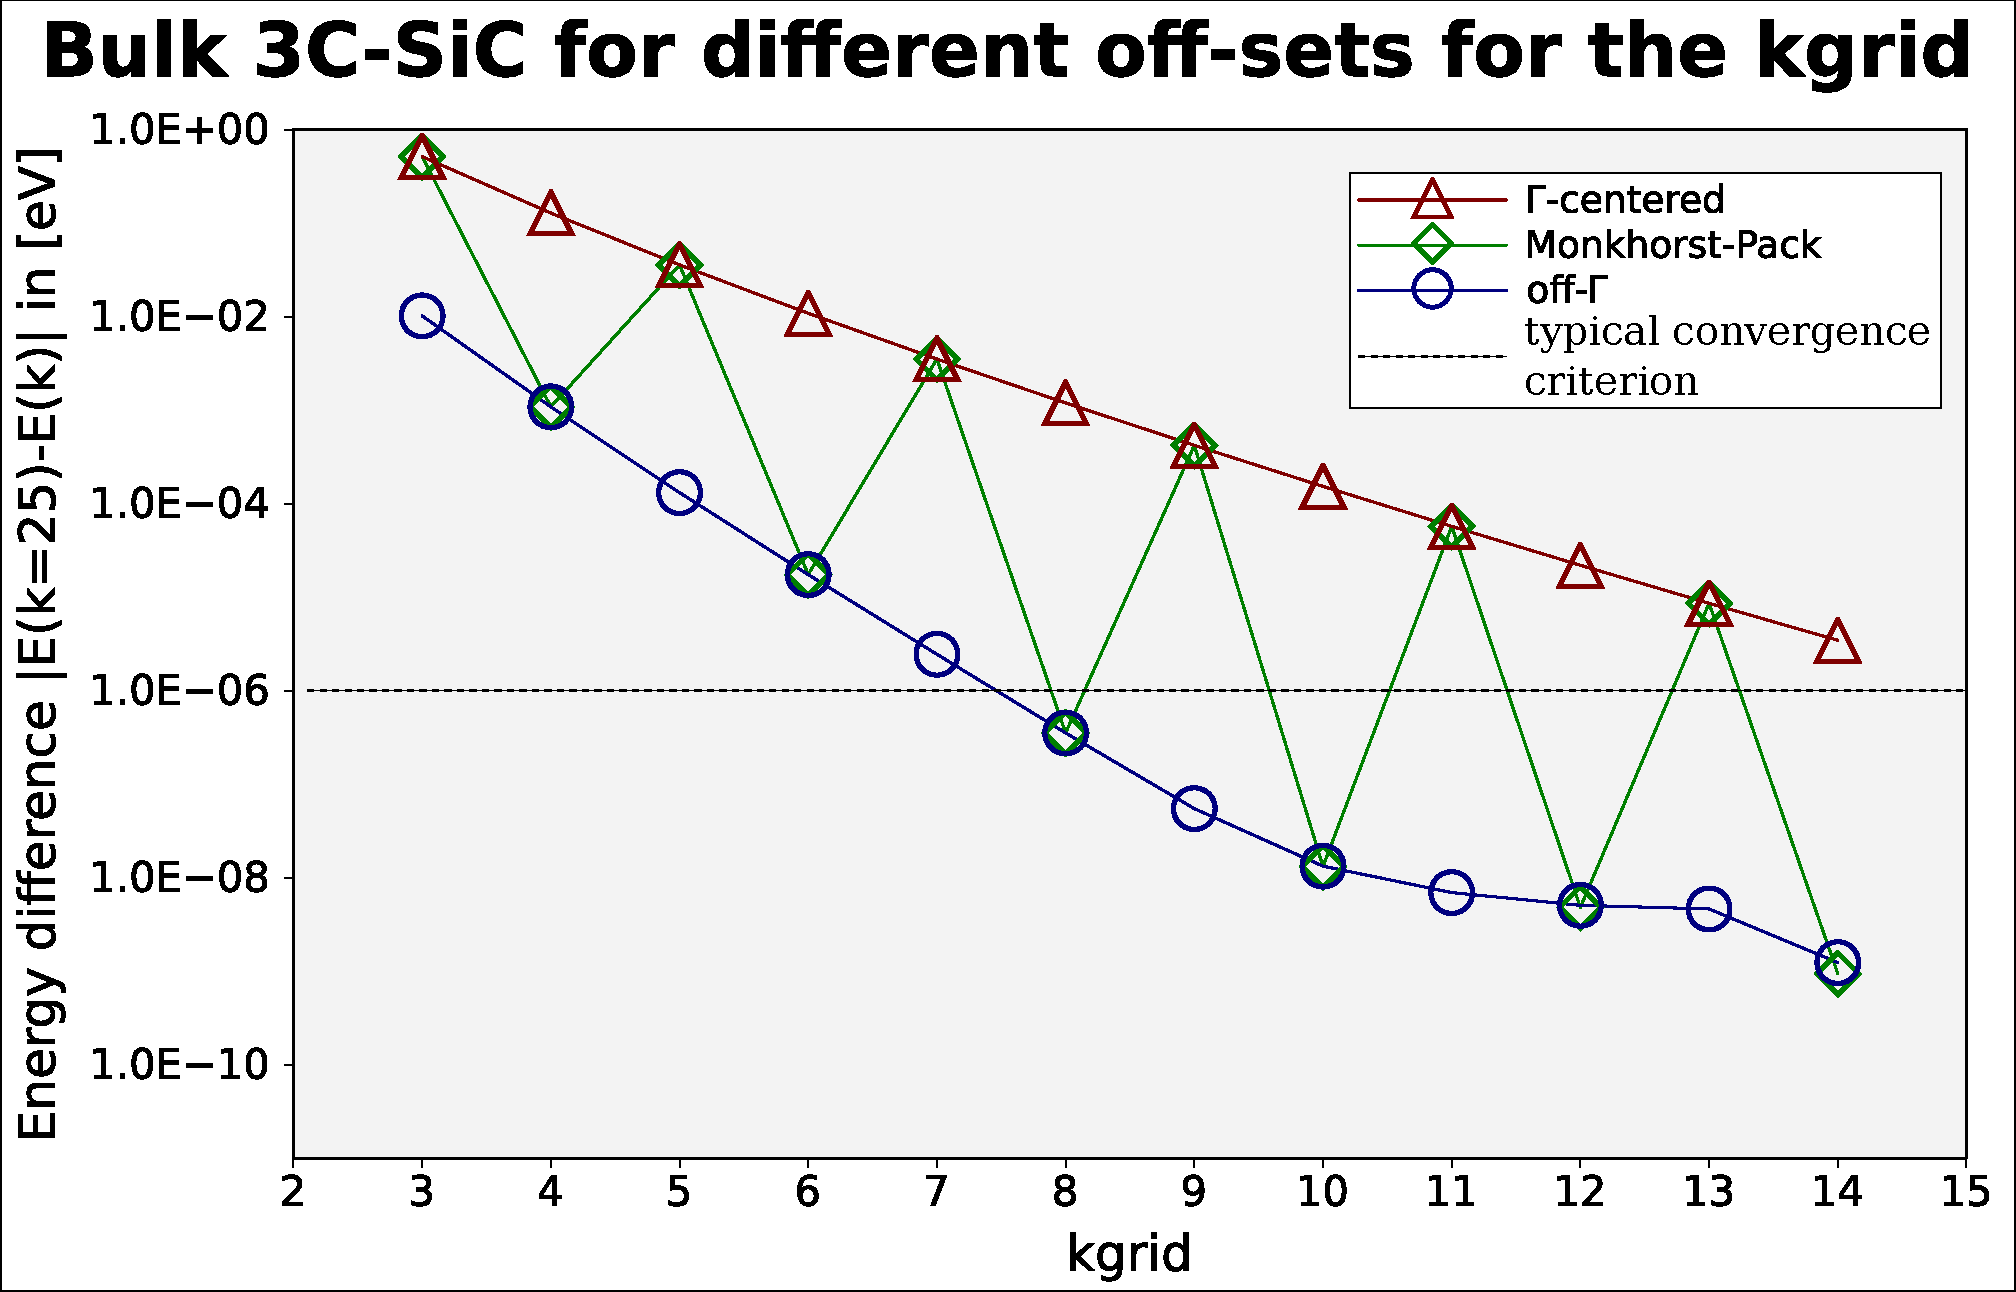
\includegraphics[width=0.80\textwidth]{./kgrid_plot_man.pdf}
 % kgrid_plot_man.pdf: 817x620 pixel, 72dpi, 28.82x21.87 cm, bb=0 0 817 620
 \caption{The $k$-grid was tested with respect to the grid density and the shift of the grid in reciprocal space. The shifts are defined in Eqn.~(\ref{eqn_K-shift}).}
 \label{fig:aims_kgrid}
\end{figure}%
%
\newpage
%
\begin{wrapfigure}[17]{r}{0.50\textwidth}
\centering
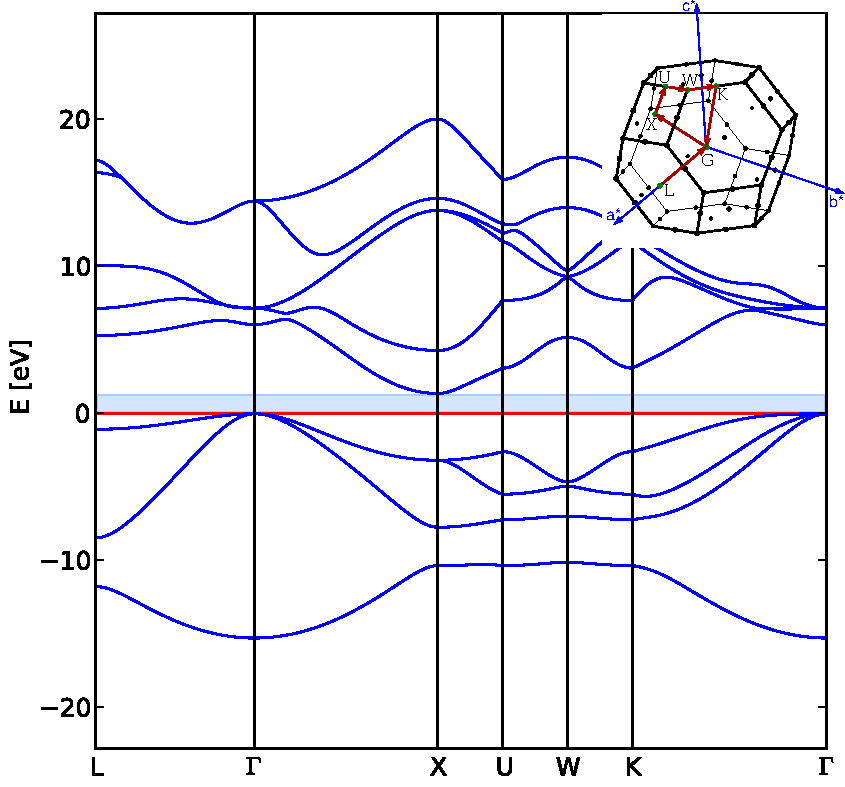
\includegraphics[width=0.45\textwidth]{./3C-SiC_bands.pdf}
% 3C-SiC_bands.pdf: 0x0 pixel, 0dpi, nanxnan cm, bb=
 \caption{The band structure of 3C-SiC with tight, Tier 2 basis settings.}
 \label{fig:3C-SiC_bands}
\end{wrapfigure}%
%
A typical convergence criterion for the total energy is a value of $10^{-6}$ eV. In Fig.~(\ref{fig:aims_kgrid}) the dashed line marks the convergence criterion. In the case of an off-$\Gamma$ shift the calculation is well converged with a $k$-grid of $8 \times 8 \times 8$. For a $\Gamma$-centered grid the calculation did not reach convergence with a grid of $14 \times 14 \times 14$. As mentioned before, in 3C-SiC the VBM is in the $\Gamma$-point. Therefore the convergence of the total energy with respect to the density of the $k$-grid is slow for every grid including the $\Gamma$-point, because the contribution of the energy in the $\Gamma$-point is over-weighted. 
In this case the off-$\Gamma$ shift gives best convergence.\\
We note the above conclusion is mainly applicable for semiconductors. In a metal, the sampling of the Fermi-surface is crucial, this demands a high $k$-grid density rather than a special off-set.  


% For emacs:
%%% Local Variables: 
%%% mode: latex
%%% TeX-master: "FHI-aims"
%%% End: 
